\section{ST-structures and HDAs}
\label{sec:st-structure-and-hda}

    For ST-structures to precisely identify events in higher-dimensional automata we need a way of translating ST-structures into higher-dimensional automata. Johansen in \cite{Johansen16STstruct} provides a way of translating ST-structures into higher-dimensional automata as follows.

    \begin{definition}[$\allST$ to $\allHDA$ \cite{Johansen16STstruct}]
        \label{def:ST-structures-to-HDA}
        We define a mapping $\stintoh : \allST \rightarrow \allHDA$ from ST-structures into $\HDA$s which for an $\ST=(E,ST,l)$ with the events linearly ordered as a list $\evlist{E}$ (that is, each event being indexed by a natural number, as in a sequence) returns the $\HDA$ $\stintoh(\ST)$ which
    
        \begin{itemize}
            \item has cells $\mathcal{Q} = \{q^{(\mathcal{S},\mathcal{T})}\in \mathcal{Q}_{n} \mid (\mathcal{S},\mathcal{T})\in ST \mbox{ and } |\mathcal{S} \setminus \mathcal{T}|=n\}$;
            \item for any two cells $q^{(\mathcal{S},\mathcal{T})}$ and $q^{(S\setminus e,T)}$ add the map entry $s_{i}(q^{(\mathcal{S},\mathcal{T})})=q^{(\mathcal{S} \setminus e,\mathcal{T})}$ where $i$ is the index of the event $e$ in the listing $\evlist{E}\!\!\downarrow_{(\mathcal{S} \setminus \mathcal{T})}$;
            \item for any two cells $q^{(\mathcal{S},\mathcal{T})}$ and $q^{(\mathcal{S},\mathcal{T} \cup e)}$ add the map entry $t_{i}(q^{(\mathcal{S},\mathcal{T})})=q^{(\mathcal{S},\mathcal{T} \cup e)}$ where $i$ is the index of the event $e$ in the listing $\evlist{E}\!\!\downarrow_{(\mathcal{S} \setminus \mathcal{T})}$;
            \item has labelling $l(q^{(\mathcal{T} \cup e,\mathcal{T})})=l(e)$ for any $q^{(\mathcal{T} \cup e,\mathcal{T})}\in \mathcal{Q}_{1}$.
        \end{itemize}

        More precisely, by $\evlist{E}\!\!\downarrow_{(\mathcal{S} \setminus \mathcal{T})}$ we represent the listing of the events in $\mathcal{S} \setminus \mathcal{T}$, namely, a list of dimension $|\mathcal{S} \setminus \mathcal{T}|$ obtained from the original listing $\evlist{E}$ by removing all other events. This new listing has the events of $\mathcal{S} \setminus \mathcal{T}$ in the same original order but with new indexes attached (ranging from $1$ to $|\mathcal{S} \setminus \mathcal{T}|$).
    \end{definition}

    As shown in \cite[Theorem 3.36]{Johansen16STstruct}, the mapping $\stintoh$ associates a rooted, connected, and adjacent-closed ST-structure with $\stintoh(\ST)$, which is a higher-dimensional automaton respecting the precubical identities and is acyclic. The non-degenerate property of higher-dimensional automata is defined by the underlying precubical set. Hence, the property of non-degeneracies is preserved. As shown by Johansen in \cite[Lemma 3.37]{Johansen16STstruct}, the way the events are picked in the definition of the mapping $\stintoh$ do not matter.


    Higher-dimensional automata are not good at identifying events and can be demonstrated by Example \ref{exp:asymmetric-conflict}, which represents the \emph{asymmetric conflict}. However, higher-dimensional automata can be faithfully represented as ST-structures which can precisely identify events.

    %The example is taken from \cite{Johansen16STstruct}, however, the example is well known and widely used in the literature \cite{Johansen16STstruct, GlabbeekP09configStruct, Pratt03trans_cancel}.

    \begin{example}[Strong asymmetric conflict]
        \label{exp:asymmetric-conflict}
        This example is taken from \cite[Example 3.38]{Johansen16STstruct}, but can also be found in \cite[Example 3]{GlabbeekP09configStruct}, and in \cite[page.22]{Pratt03trans_cancel} the asymmetric conflict is considered \emph{strong}. 
    
        %This example shows the gain in expressive power of the ST-structure over pure event structures, hence configurations structures. We have only considered prime event structures in this thesis, however, they are similar to pure event structures in \cite[Definition 1.5]{GlabbeekP09configStruct}. The asymmetric conflict can be captured by the unrestricted event structure of \cite{GlabbeekP09configStruct}, which is an extension of prime event structure with a binary conflict relation. Also, asymmetric conflict can be captured by the adjacent-closed ST-structure of Figure \ref{fig:asymmetric-conflict-st-hda} (left).
    
        \begin{figure}[ht]
            \centering
            \includegraphics[scale=0.9]{Figures/4.Relationship-with-other-models-of-concurrency/ST-structure-and-HDA/Asymmetric-conflict.pdf}
            \captionof{figure}[Asymmetric conflict]{Example of ST-structures and higher-dimensional automata representing the asymmetric conflict $a + b$. The higher-dimensional automaton (left) is isomorphic to the higher-dimensional automaton (right). On the other hand, we see that the ST-structure (left) is not isomorphic to the ST-structure (right). Since, the ST-structure (left) is on two events and the ST-structure (right) is on three events.}
            \label{fig:asymmetric-conflict-st-hda}
        \end{figure}
    
        The example has no concurrency and involves two events, imposing the only restriction that once event $a$ happens, then event $b$ cannot occur anymore. 
    
        %The notion of asymmetric conflict for event structures has been studied by Baldan et al. in \cite{Baldan01AsymmetricES}.
    
        Higher-dimensional automata are not good at identifying the particular events, making the representation of the example as a higher-dimensional automaton challenging. Higher-dimensional automata are state-based models that represent events by actions, where actions are labels for the particular events. These actions may occur multiple times, where events only occur once in an execution. The standard way of identifying events in higher-dimensional is by equivalence classes of transitions, where two transitions are equivalent when they are parallel in the boundary of a filled square, see Figure \ref{fig:HDA-filled-interleaving-square}.
    
        The equivalence classes of transitions for higher-dimensional automata, shown in Figure \ref{fig:asymmetric-conflict-st-hda} (left), would not result in the corresponding 2-event ST-structure, which is what we want. However, would result in the 3-event ST-structure of Figure \ref{fig:asymmetric-conflict-st-hda} (right). The 2-event ST-structure is not isomorphic to the 3-event ST-structure. On the other hand, the two representations of the higher-dimensional automata from Figure \ref{fig:asymmetric-conflict-st-hda} (left and right) are isomorphic.
    \end{example}

%\begin{example}[Strong asymmetric conflict]\label{exp:asymmetric-conflict}
%This example, taken from \cite[Ex .3]{GlabbeekP09configStruct} (called \textit{strong} in \cite[p.22]{Pratt03trans_cancel}), shows the gain in expressive power of the ST-structures. Asymmetric conflict cannot be captured in the \emph{pure event structures} of \cite[Def.1.5]{GlabbeekP09configStruct}, hence not by the configuration structures. Asymmetric conflict can be captured by the unrestricted event structures of \cite{GlabbeekP09configStruct}, and thus, also by the adjacent-closed ST-structure of Fig.~\ref{fig:asymmetric-conflict-st-hda} (left).

%\begin{figure}[ht]
%        \centering
%        \includegraphics[scale=0.9]{Figures/4.Relationship-with-other-models-of-concurrency/ST-structure-and-HDA/Asymmetric-conflict.pdf}
%         \captionof{figure}[Asymmetric conflict]{asymmetric conflict of HDA and ST.}
%        \label{fig:asymmetric-conflict-st-hda}
%    \end{figure}

%The example has no concurrency and involves two events, imposing the only restriction that once event $s$ happens, event $b$ cannot happen any more. The notion of \emph{asymmetric conflict} for even structures has been studies in \cite{Baldan01AsymmetricES}.

%Within $\HDA$ it is more cumbersome to represent this example because $\HDA$ are not good at identifying the particular events. $\HDA$ abstract from the concrete events and concentrate only on the labels. 
%The standard way of identifying events is by equivalence classes of transitions, where two transitions are equivalent when they are parallel in the boundary of a filled square (i.e., what we assumed until now in our $\HDA$ examples).


%Applying this technique to the $\HDA$ in Figure ~\ref{fig_ex_asymconflict1}(middle) would not result in the corresponding 2-events ST-structure (which is what we want), but would result in the 3-events ST-structure of Fig.~\ref{fig_ex_asymconflict1}(right), and these two ST-structures are not isomorphic.
%On the other hand, the two representations of $\HDA$ from Fig.~\ref{fig_ex_asymconflict1}(middle and right) are isomorphic. 
%Nevertheless, if we are interested in representing systems only up to hh-bisimulation, then both $\HDA$ and ST-structures are as good, because the different representations of ST-structures (with 2 or 3 events) would be equated by the hh-bisimulation.
%\end{example}


%From Example \ref{exp:asymmetric-conflict}, we see that non-isomorphic ST-structures collapse into isomorphic higher-dimensional automata. A proof for Proposition \ref{prop:ST-structure-to-HDA-isomorphism}, taken from \cite[Proposition 3.39]{Johansen16STstruct}, is shown by Johansen, where the mapping $\stintoh$ either preserves isomorphism or collapses non-isomorphic ST-structures into isomorphic higher-dimensional automata. We will provide the proof by Johansen found in \cite[Proposition 3.39]{Johansen16STstruct}.

%\begin{proposition}\
%\label{prop:ST-structure-to-HDA-isomorphism}
%    \begin{enumerate}
%        \item\label{prop_stintoh_iso_1} The mapping $\stintoh$ from Definition~\ref{def:ST-structures-to-HDA} preserves isomorphism
%        \[
%            \mbox{for } \ST \isomorphic \ST' \mbox{ then } \stintoh(\ST) \isomorphic \stintoh(\ST').
%        \]
%        \item\label{prop_stintoh_iso_collapse} The mapping $\stintoh$ may collapse non-isomorphic ST-structures into isomorphic $\HDA$.
%    \end{enumerate}
%\end{proposition}
    
    In \cite[Proposition 3.39]{Johansen16STstruct}, the mapping $\stintoh$ from Definition~\ref{def:ST-structures-to-HDA} preserves isomorphism. However, it may collapse non-isomorphic ST-structures into isomorphic higher-dimensional automata. Consider the two ST-structures from Figure~\ref{fig:asymmetric-conflict-st-hda} which are not isomorphic since the left one is defined by two events while the right one is defined by three events, whereas the higher-dimensional automata that the mapping $\stintoh$ associates are isomorphic. This means that $\stintoh$ is not an embedding from $\allST$ to $\allHDA$ since it looses information, namely, the events. A natural question to raise is if a mapping from $\allHDA$ to $\allST$ is then an embedding from $\allHDA$ to $\allST$. We will first define a mapping from $\allHDA$ to $\allST$.

    \begin{definition}[$\allHDA$ to $\allST$ \cite{Johansen16STstruct}]
        \label{def:HDA-to-ST-structure}
        Consider a non-degenerate $\HDA$ $H=(\mathcal{Q},\overline{s},\overline{t},l,I)$. Define a relation $\eventEquivHDAs\subseteq \mathcal{Q}_{1}\times \mathcal{Q}_{1}$ on transitions as 
    
        \[
            q_{1}\eventEquivHDAs q_{1}' \mbox{\hspace{2ex} iff \hspace{2ex}} \exists q_{2}\in \mathcal{Q}_{2}:\alpha_{i}(q_{2})=q_{1}\wedge \beta_{i}(q_{2})=q_{1}'
        \]

        for some $i\leq 2$ and $\alpha,\beta\in\{s,t\}$. Consider the reflexive and transitive closure of the above relation, and denote it the same. This is now an equivalence relation on $\mathcal{Q}_{1}$. Consider an equivalence class $\equivClass{q_{1}}$ to be all $q_{1}'$ equivalent with $q_{1}$. Such an equivalence class is called \emph{an event}.

        Define a map $\ST:\allHDA \rightarrow \allST$ which builds an ST-structure $\ST(H)$ by associating to each rooted path $\pi\in H$ an ST-configuration as follows.

        \begin{enumerate}
            \item\label{hintost_1} for the minimal rooted path which ends in $I$ associate $(\emptyset,\emptyset)$;
            \item\label{hintost_2} for any path $\pi$ which ends in a transition $\finishPath{\pi}=q_{1}\in \mathcal{Q}_{1}$ then 
        
            \begin{enumerate}
                \item\label{hintost_21} add the ST-configuration $\hintost(\pi)=\hintost(\pi_{s})\cup(\equivClass{q_{1}},\emptyset)$, where $\pi_{s}$ is a shorter path reaching through an s-map the homotopy class of $\pi$, that is, $\pi_{s}\transition{s}q_{1}\in\homotopyClass{\pi}$;
                \item\label{hintost_22} add the ST-configuration $\hintost(\pi\transition{t}q_{0})=\hintost(\pi)\cup(\emptyset,\equivClass{q_{1}})$;
            \end{enumerate}

            \item\label{hintost_3} for any path $\pi$ which ends in a higher cell $\finishPath{\pi}=q_{n}\in \mathcal{Q}_{n}$, with $n\geq 2$, then add the ST-configuration $\hintost(\pi)=\hintost(\pi^{i})\cup\hintost(\pi^{j})$, with $\pi^{i}\neq\pi^{j}$, $\pi^{i}\transition{s}q_{n}\in\homotopyClass{\pi}$, and $\pi^{j}\transition{s}q_{n}\in\homotopyClass{\pi}$.
        \end{enumerate}
    \end{definition}

    As shown in \cite[Proposition 3.42]{Johansen16STstruct}, the mapping $\ST$ associates an acyclic and non-degenerate higher-dimensional automata with $\ST(H)$, which is a rooted, connected, and adjacent-closed ST-structure. Furthermore, in \cite[Proposition 3.44]{Johansen16STstruct}, the mapping $\ST$ from Definition~\ref{def:HDA-to-ST-structure} preserves isomorphism of reachable parts. However, it may collapse non-isomorphic higher-dimensional automata into isomorphic ST-structures. This can be seen by considering the two higher-dimensional automata from Figure \ref{fig:Unfolding-HDA}, which are translated into the same ST-structure by $\ST$. The mapping $\ST$ considers the two higher-dimensional automata which are not isomorphic to be two ST-structures which are isomorphic. The higher-dimensional automata are not isomorphic since the right one has a split corner whereas the left one is a square with its faces nicely placed, forming a complete square. 
    
    
        
    %    \begin{figure}[ht]
    %        \centering
    %        \includegraphics[scale=0.9]{Figures/4.Relationship-with-other-models-of-concurrency/ST-structure-and-HDA/HDA-collapse-triangle.pdf}
    %        \captionof{figure}[History unfolding of a triangular $\HDA$ through $\hintost$]{Example of ST-structures and higher-dimensional automata representing the unfoldings of a triangular $\allHDA$ through $\hintost$. The ST-structure (left) is isomorphic to ST-structure (right). On the other hand, we see the higher-dimensional automaton (right) is not isomorphic to the higher-dimensional automaton (left). Since, the higher-dimensional automaton (left) has a split corner and the higher-dimensional automaton (right) is a nicely shaped square.}
    %        \label{fig:Unfolding-triangle-HDA}
    %    \end{figure}
        
    \begin{figure}[ht]
        \centering
        \includegraphics[scale=0.9]{Figures/4.Relationship-with-other-models-of-concurrency/ST-structure-and-HDA/HDA-collapse.pdf}
        \captionof{figure}[History unfolding of a square $\HDA$ through $\hintost$]{Example of ST-structures and higher-dimensional automata representing the unfoldings of a square $\HDA$ through $\hintost$. The ST-structure (left) is isomorphic to ST-structure (right). On the other hand, we see the higher-dimensional automaton (right) is not isomorphic to the higher-dimensional automaton (left). Since, the higher-dimensional automaton (right) has a split corner and the higher-dimensional automaton (left) is a nicely shaped square.}
        \label{fig:Unfolding-HDA}
    \end{figure}
    
    The mapping $\ST$ is not an embedding from $\allHDA$ to $\allST$ since it looses information, which is the mappings ability to announce the difference between when $a$ happens before $b$, or $b$ happens before $a$. In other words, being able to see the difference between the split corner of a square and a nicely shaped square.



    %\ctlong{Add the things I need from the Journal here. ST-paper. Include the Assymetrical conflict. That this cannot be done with HDAs, but faithfully done with ST-structures.}

    %\section*{Broken box example}

    %This is the example of van Glabbeek [3, Fig.11], pictured here in Figure x, with the cube with one face missing, and its strange looking unfolding where the corner is split into two.

    %\ctlong{edit the model to be more similar to the example provided in \cite{Johansen16STstruct}}
    %\documentclass[tikz,border=10pt]{standalone}
\begin{document}
  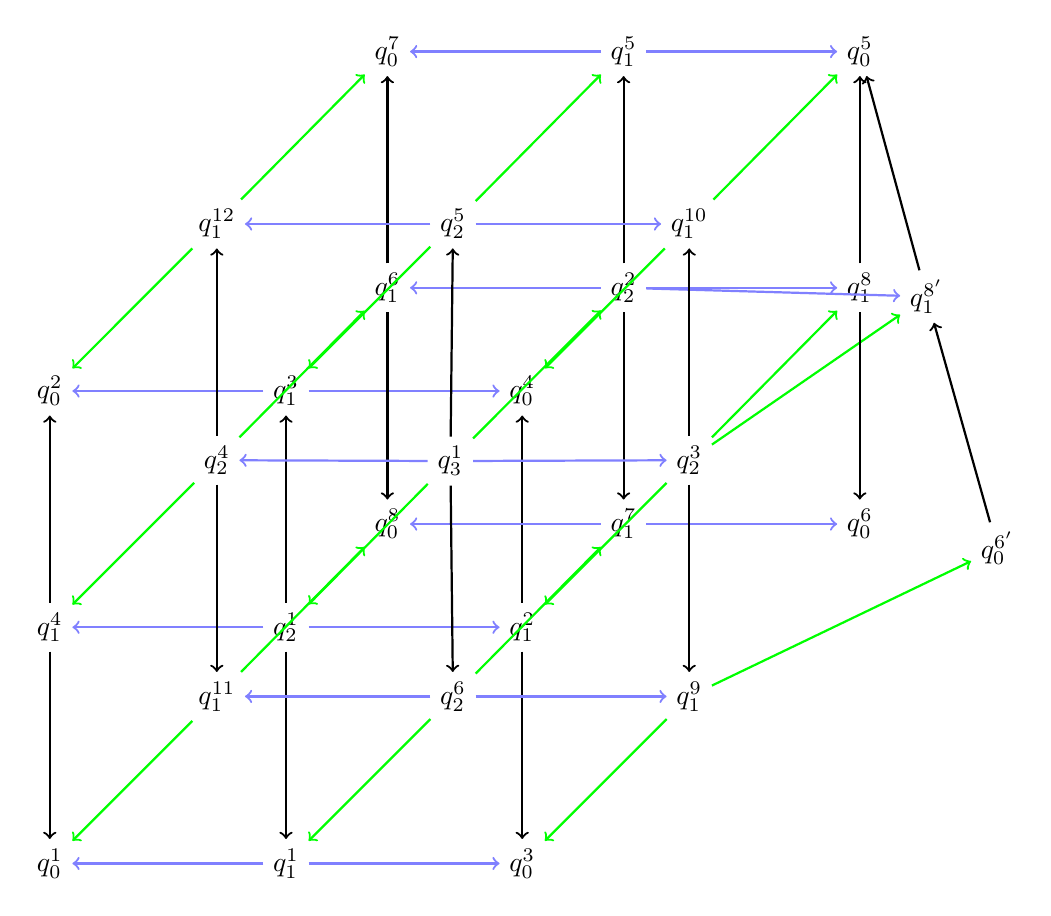
\begin{tikzpicture}[node distance=3cm, align=center]
    \title{unfolded HDA}
    % face 1
    \node(q01)                  {$q^{1}_{0}$};
    \node(q11) [right of=q01]   {$q^{1}_{1}$};
    \node(q14) [above of=q01]   {$q^{4}_{1}$};
    \node(q03) [right of=q11]   {$q^{3}_{0}$};
    \node(q02) [above of=q14]   {$q^{2}_{0}$};
    \node(q12) [above of=q03]   {$q^{2}_{1}$};
    \node(q04) [above of=q12]   {$q^{4}_{0}$};
    \node(q13) [right of=q02]   {$q^{3}_{1}$};
    \node(q21) [right of=q14]   {$q^{1}_{2}$};
    
    % face 2
    \node(q08) [above right=4cm] {$q^{8}_{0}$};
    \node(q17) [right of=q08] {$q^{7}_{1}$};
    \node(q16) [above of=q08] {$q^{6}_{1}$};
    \node(q06) [right of=q17] {$q^{6}_{0}$};

    \node(q07) [above of=q16] {$q^{7}_{0}$};
    \node(q18) [above of=q06] {$q^{8}_{1}$};
    \node(q05) [above of=q18] {$q^{5}_{0}$};
    \node(q15) [right of=q07] {$q^{5}_{1}$};
    \node(q22) [right of=q16] {$q^{2}_{2}$};

    %face 3
    \node(q110) [above right of=q04] {$q^{10}_{1}$};
    \node(q19) [above right of=q03] {$q^{9}_{1}$};
    \node(q23) [above right of=q12] {$q^{3}_{2}$};

    %face 4
    \node(q111) [above right of=q01] {$q^{11}_{1}$};
    \node(q112) [above right of=q02] {$q^{12}_{1}$};
    \node(q24) [above right of=q14] {$q^{4}_{2}$};

    %face 5
    \node(q25) [right of=q112] {$q^{5}_{2}$};

    %face 6
    \node(q26) [right of=q111] {$q^{6}_{2}$};


    %3D
    \node(q31) [above right=4.8cm] {$q^{1}_{3}$};

    %extra
    \node(q06x) [above=4cm, right=11.7cm] {$q^{6'}_{0}$};
    \node(q18x) [above=7.2cm, right=10.8cm] {$q^{8'}_{1}$};

    \draw [->][draw=black, thick] (q06x) to node [below] {} (q18x);
    \draw [->][draw=black, thick] (q18x) to node [left] {} (q05);
    \draw [->][draw=blue!50, thick] (q22) to node [left] {} (q18x);
    \draw [->][draw=green, thick] (q23) to node [left] {} (q18x);


    %%%%% Edges Figure 1 %%%%%
    %face 1(1D)
    \draw [->][draw=blue!50, thick] (q11) to node [below] {} (q01);
    \draw [->][draw=black, thick] (q14) to node [left] {} (q01);
    \draw [->][draw=blue!50, thick] (q11) to node [below] {} (q03);
    \draw [->][draw=black, thick] (q14) to node [left] {} (q02);
    \draw [->][draw=black, thick] (q12) to node [right] {} (q03);
    \draw [->][draw=black, thick] (q12) to node [right] {} (q04);
    \draw [->][draw=blue!50, thick] (q13) to node [above] {} (q02);
    \draw [->][draw=blue!50, thick] (q13) to node [above] {} (q04);

    %(2D)
    \draw [->][draw=blue!50, thick] (q21) to node [below] {} (q14);
    \draw [->][draw=black, thick] (q21) to node [left] {} (q11);
    \draw [->][draw=blue!50, thick] (q21) to node [below] {} (q12);
    \draw [->][draw=black, thick] (q21) to node [left] {} (q13);

    %face 2(1D)
    \draw [->][draw=blue!50, thick] (q17) to node [below] {} (q08);
    \draw [->][draw=black, thick] (q16) to node [left] {} (q08);
    \draw [->][draw=blue!50, thick] (q17) to node [below] {} (q06);
    \draw [->][draw=black, thick] (q16) to node [left] {} (q07);
    \draw [->][draw=black, thick] (q18) to node [right] {} (q06);
    \draw [->][draw=black, thick] (q18) to node [right] {} (q05);
    \draw [->][draw=blue!50, thick] (q15) to node [above] {} (q07);
    \draw [->][draw=blue!50, thick] (q15) to node [above] {} (q05);    

    %(2D)
    \draw [->][draw=blue!50, thick] (q22) to node [below] {} (q16);
    \draw [->][draw=black, thick] (q22) to node [left] {} (q17);
    \draw [->][draw=black, thick] (q22) to node [left] {} (q15);
    \draw [->][draw=blue!50, thick] (q22) to node [below] {} (q18);

    %face 3(1D)
    \draw [->][draw=green, thick] (q110) to node [right] {} (q04);
    \draw [->][draw=green, thick] (q110) to node [right] {} (q05);
    \draw [->][draw=green, thick] (q19) to node [above] {} (q03);
    \draw [->][draw=green, thick] (q19) to node [above] {} (q06x);    

    %(2D)
    \draw [->][draw=green, thick] (q23) to node [below right] {} (q12);
    \draw [->][draw=black, thick] (q23) to node [left] {} (q19);
    \draw [->][draw=black, thick] (q23) to node [left] {} (q110);
    \draw [->][draw=green, thick] (q23) to node [below right] {} (q18);    

    %face 4(1D)
    \draw [->][draw=green, thick] (q112) to node [right] {} (q02);
    \draw [->][draw=green, thick] (q112) to node [right] {} (q07);
    \draw [->][draw=green, thick] (q111) to node [above] {} (q01);
    \draw [->][draw=green, thick] (q111) to node [above] {} (q08);    

    %(2D)
    \draw [->][draw=green, thick] (q24) to node [below right] {} (q14);
    \draw [->][draw=black, thick] (q24) to node [left] {} (q111);
    \draw [->][draw=black, thick] (q24) to node [left] {} (q112);
    \draw [->][draw=green, thick] (q24) to node [below right] {} (q16);

    %face 5(2D)
    \draw [->][draw=blue!50, thick] (q25) to node [below right] {} (q112);
    \draw [->][draw=green, thick] (q25) to node [left] {} (q13);
    \draw [->][draw=blue!50, thick] (q25) to node [left] {} (q110);
    \draw [->][draw=green, thick] (q25) to node [below right] {} (q15);


    %face 6(2D)
    \draw [->][draw=blue!50, thick] (q26) to node [below right] {} (q111);
    \draw [->][draw=green, thick] (q26) to node [left] {} (q11);
    \draw [->][draw=green, thick] (q26) to node [left] {} (q17);
    \draw [->][draw=blue!50, thick] (q26) to node [below right] {} (q19);

    %3D
    \draw [->][draw=green, thick] (q31) to node [below right] {} (q21);
    \draw [->][draw=green, thick] (q31) to node [left] {} (q22);
    \draw [->][draw=blue!50, thick] (q31) to node [left] {} (q23);
    \draw [->][draw=blue!50, thick] (q31) to node [left] {} (q24);
    \draw [->][draw=black, thick] (q31) to node [left] {} (q25);
    \draw [->][draw=black, thick] (q31) to node [below right] {} (q26);

    %face 1
    %\draw [->][draw=black, thick] (q11) to node [below] {$s_{1}$} (q01);
    %\draw [->][draw=black, thick] (q14) to node [left] {$s_{1}$} (q01);
    %\draw [->][draw=black, thick] (q11) to node [below] {$t_{1}$} (q03);
    %\draw [->][draw=black, thick] (q14) to node [left] {$t_{1}$} (q02);
    %\draw [->][draw=black, thick] (q12) to node [right] {$s_{1}$} (q03);
    %\draw [->][draw=black, thick] (q12) to node [right] {$t_{1}$} (q04);
    %\draw [->][draw=black, thick] (q13) to node [above] {$s_{1}$} (q02);
    %\draw [->][draw=black, thick] (q13) to node [above] {$t_{1}$} (q04);

    %face 1
    %\draw [->][draw=green, thick] (q21) to node [below] {$s_{2}$} (q14);
    %\draw [->][draw=green, thick] (q21) to node [left] {$s_{2}$} (q11);
    %\draw [->][draw=green, thick] (q21) to node [below] {$t_{2}$} (q12);
    %\draw [->][draw=green, thick] (q21) to node [left] {$t_{2}$} (q13);

    %face 2
    %\draw [->][draw=black, thick] (q17) to node [below] {$s_{1}$} (q08);
    %\draw [->][draw=black, thick] (q16) to node [left] {$s_{1}$} (q08);
    %\draw [->][draw=black, thick] (q17) to node [below] {$t_{1}$} (q06);
    %\draw [->][draw=black, thick] (q16) to node [left] {$t_{1}$} (q07);
    %\draw [->][draw=black, thick] (q18) to node [right] {$s_{1}$} (q06);
    %\draw [->][draw=black, thick] (q18) to node [right] {$t_{1}$} (q05);
    %\draw [->][draw=black, thick] (q15) to node [above] {$s_{1}$} (q07);
    %\draw [->][draw=black, thick] (q15) to node [above] {$t_{1}$} (q05);    

    %\draw [->][draw=green, thick] (q22) to node [below] {$s_{2}$} (q16);
    %\draw [->][draw=green, thick] (q22) to node [left] {$s_{2}$} (q17);
    %\draw [->][draw=green, thick] (q22) to node [left] {$t_{2}$} (q15);
    %\draw [->][draw=green, thick] (q22) to node [below] {$t_{2}$} (q18);

    %face 3
    %\draw [->][draw=black, thick] (q110) to node [right] {$s_{1}$} (q04);
    %\draw [->][draw=black, thick] (q18) to node [right] {$t_{1}$} (q05);
    %\draw [->][draw=black, thick] (q15) to node [above] {$s_{1}$} (q07);
    %\draw [->][draw=black, thick] (q15) to node [above] {$t_{1}$} (q05);    

    %\draw [->][draw=green, thick] (q23) to node [below right] {$s_{2}$} (q12);
    %\draw [->][draw=green, thick] (q23) to node [left] {$s_{2}$} (q19);
    %\draw [->][draw=green, thick] (q23) to node [left] {$t_{2}$} (q110);
    %\draw [->][draw=green, thick] (q23) to node [below right] {$t_{2}$} (q18);    


    %%%% Labels Figure 1 %%%%

    %face 1
    %\draw [->][draw=black, thick] (q11) to node [above] {a} (q01);
    %\draw [->][draw=black, thick] (q14) to node [right] {b} (q01);
    %\draw [->][draw=black, thick] (q11) to node [above] {a} (q03);
    %\draw [->][draw=black, thick] (q14) to node [right] {b} (q02);
    %\draw [->][draw=black, thick] (q12) to node [left] {b} (q03);
    %\draw [->][draw=black, thick] (q12) to node [left] {b} (q04);
    %\draw [->][draw=black, thick] (q13) to node [below] {a} (q02);
    %\draw [->][draw=black, thick] (q13) to node [below] {a} (q04);

    %\draw [->][draw=green, thick] (q21) to node [above] {a} (q14);
    %\draw [->][draw=green, thick] (q21) to node [right] {b} (q11);
    %\draw [->][draw=green, thick] (q21) to node [above] {a} (q12);
    %\draw [->][draw=green, thick] (q21) to node [right] {b} (q13);

    %face 2
    %\draw [->][draw=black, thick] (q17) to node [above] {a} (q08);
    %\draw [->][draw=black, thick] (q16) to node [right] {b} (q08);
    %\draw [->][draw=black, thick] (q17) to node [above] {a} (q06);
    %\draw [->][draw=black, thick] (q16) to node [right] {b} (q07);
    %\draw [->][draw=black, thick] (q18) to node [left] {b} (q06);
    %\draw [->][draw=black, thick] (q18) to node [left] {b} (q05);
    %\draw [->][draw=black, thick] (q15) to node [below] {a} (q07);
    %\draw [->][draw=black, thick] (q15) to node [below] {a} (q05);

    %\draw [->][draw=green, thick] (q22) to node [above left] {a} (q16);
    %\draw [->][draw=green, thick] (q22) to node [right] {b} (q17);
    %\draw [->][draw=green, thick] (q22) to node [right] {b} (q15);
    %\draw [->][draw=green, thick] (q22) to node [above left] {a} (q18);

    %face 3

    %\draw [->][draw=green, thick] (q23) to node [above] {a} (q12);
    %\draw [->][draw=green, thick] (q23) to node [right] {b} (q19);
    %\draw [->][draw=green, thick] (q23) to node [right] {b} (q110);
    %\draw [->][draw=green, thick] (q23) to node [above] {a} (q18);






  \end{tikzpicture}
\end{document}

    %Just a quick draft before the end of the day:

    %As part of the example given by van Glabbeek, it provides the idea of having the possibility to exclude the mutual exclusive based on the order action A, B and C occur. A and B are two computer scientist competing to get to the podium and at the middle there is an obstacle which prevents both of them run at the same time. Also, we have an independent person C which removes the obstacle to allow A and B to run independently. If A passes the obstacle before B, or vice versa, then a last person D, or E, is to give an announcement preventing C from removing the obstacle.

    %\ctlong{Draw up the new model of the broken box. (check)}
    %\ctlong{Write an introduction to the broken box example.}
    %\ctlong{Explain the problem that arises from the example.
    %	- non-isomorphic HDA into isomorphic ST-structures.
    %	- hereditary history preserving HDA.}


    %We have now the figure 6 left(broken box) and a new figure(upside box). When we do the unfolding of the upside box, we get the broken box. We can see that the upside box is a sculpture, but its unfolding is not.

    In Figure \ref{fig:asymmetric-conflict-st-hda}, we can see that higher-dimensional automata are not able to precisely identify events, but can be faithfully interpreted as ST-structures. ST-structures are able to precisely capture events while events in higher-dimensional automata are not easily captured. As we have shown in Figure \ref{fig:Unfolding-HDA}, ST-structures are not able to capture the difference between a higher-dimensional automaton and the unfolding of that higher-dimensional automaton. Hence, some processes might only be able to be represent as higher-dimensional automata, and identifying precisely these events of the processes would be challenging. We are interested in finding a model that is able to capture the aspect of higher-dimensional automata, but also be faithfully translated to ST-structures. In this regard, we will investigate Chu spaces and ST-structures.